\chapter*{Chapter 1 - Introduction to vibration and free response}

  \begin{fmd-definition}{Degree of freedom}
    The degree of freedom of a system is the minimum number of displacement coordinates needed to represent the position of the systems mass at any instant of time.
  \end{fmd-definition}

  \begin{fmd-definition}{Free response}
    Free response refers to analysing the vibration of a system resulting from a non-zero inital displacement and/or velocity of the system with no external force or moment applied.
  \end{fmd-definition}

  \section{The spring-mass model}
    The fundamental kinematic quantities used to describe the motion of a particle are displacement, velocity, and acceleration vectors.

    \begin{fmd-definition}{Kinematic}
      Kinematic quantities are those that describe the motion of a particle without regard to the forces that cause the motion.
    \end{fmd-definition}

    From physics, we know that: The motion of a mass with changing velocity is determined by the net force acting on the mass.
    \begin{figure}
      \centering
      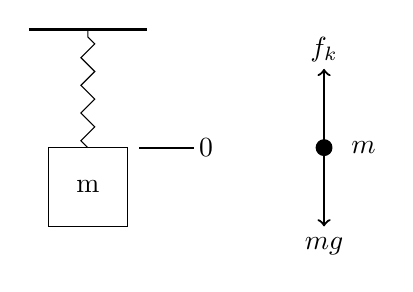
\begin{tikzpicture}
        % single DOF mass-spring system
        \draw[thick] (-0.25,2.5) -- (1.25,2.5);
        \draw (0,0) rectangle (1,1);
        \node at (0.5,0.5) {m};
        \draw[decorate,decoration=zigzag] (0.5,1) -- (0.5,2.5);
        \draw[thick] (1.15,1) -- (1.85,1);
        \node at (2,1) {0};
        % draw a point mass
        \draw[fill] (3.5,1) circle (0.1);
        \node at (4,1) {$m$};
        \draw[thick,->] (3.5,1) -- (3.5,2); % kx
        \node at (3.5,2.25) {$f_k$};
        \draw[thick,->] (3.5,1) -- (3.5,0); % mg
        \node at (3.5,-0.25) {$mg$};

      \end{tikzpicture}
      \caption{Single degree of freedom mass-spring system}\label{fig:single-dof-mass-spring}
    \end{figure}

    In~\cref{fig:single-dof-mass-spring}, the forces acting on the mass consist of the force of gravity pulling down ($mg$) and the \textit{elastic-restoring} force of the spring pulling it back up ($f_k$)\dots

    \begin{fmd-definition}{Constant of proportionality}
      The slope of the straight line in the graph of force versus displacement of a spring.
    \end{fmd-definition}

    The constant of proportionality can be easily determined for a spring using a simple experiment. Hanging a known mass on a spring and measuring the resulting displacement. This can be repeated for successivly hevier masses and a force displacement graph can be plotted.

    \begin{figure}
      \begin{tikzpicture}
        % draw a spring (zig-zag) with no mass attached and label the bottom as datum x_0
        \draw[thick] (-1.25, 0) -- (1.25, 0);
        \draw[decorate,decoration=zigzag] (0,0) -- (0,-2);
        \draw (0, -2) -- (1, -2);
        \node at (1.25,-2) {$x_0$};
        % draw a spring with a mass attached and slightly stretched label x_1
        \draw[thick] (2.5, 0) -- (5.5, 0);
        \draw[decorate,decoration=zigzag] (4,0) -- (4,-2.5);
        \draw (4, -2.5) -- (5, -2.5);
        \node at (5.5,-2.5) {$x_1$};
        \draw (3.25, -2.5) rectangle (4.75, -2.75);
        % draw a spring with a mass attached and stretched label x_2
        \draw[thick] (7, 0) -- (10, 0);
        \draw[decorate,decoration=zigzag] (8.5,0) -- (8.5,-3);
        \draw (8.5, -3) -- (9.5, -3);
        \node at (10,-3) {$x_2$};
        \draw (7.75, -3) rectangle (9.25, -3.25);
        \draw (7.75, -3.25) rectangle (9.25, -3.5);
        % draw a spring with a mass attached and stretched label x_3
        \draw[thick] (11.5, 0) -- (14.5, 0);
        \draw[decorate,decoration=zigzag] (13,0) -- (13,-3.5);
        \draw (13, -3.5) -- (14, -3.5);
        \node at (14.5,-3.5) {$x_3$};
        \draw (12.25, -3.5) rectangle (13.75, -3.75);
        \draw (12.25, -3.75) rectangle (13.75, -4);
        \draw (12.25, -4) rectangle (13.75, -4.25);

        % draw a dashed line across the picture showing the datum
        \draw[dashed] (1.5, -2) -- (14.5, -2);
      \end{tikzpicture}
      \caption{A schematic of a massless spring with no mass attached showing its static equilibrium position, followed by increments of increasing added mass illustrating the corresponding deflections.}\label{fig:spring-deflection} 
    \end{figure}

    \begin{figure}[h]
      \centering
      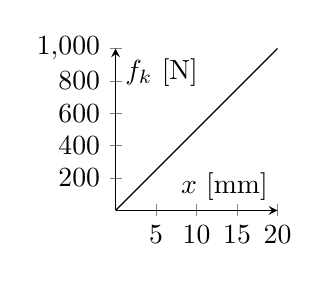
\begin{tikzpicture}
        \begin{axis}[axis lines=middle,
          xmin=0, xmax=20,
          ymin=0, ymax=1000,
          width=0.3\textwidth,
          height=0.3\textwidth,
          xlabel={$x$ [mm]},
          ylabel={$f_k$ [N]},
          ]
          % show the points
          \addplot [domain=0:1000, samples=4, color=black]{50*x};
        \end{axis}

      \end{tikzpicture}
      \caption{The static deflection curve for the spring in~\cref{fig:spring-deflection}}\label{fig:spring-deflection-curve}
    \end{figure}
      
